\hspace*{0.77in}
\includegraphics[width=0.77\textwidth]{from_HBSe_20151207T070326__124_45328_126_52461_small.png}

\tikzset{every picture/.style={line width=0.75pt}} %set default line width to 0.75pt

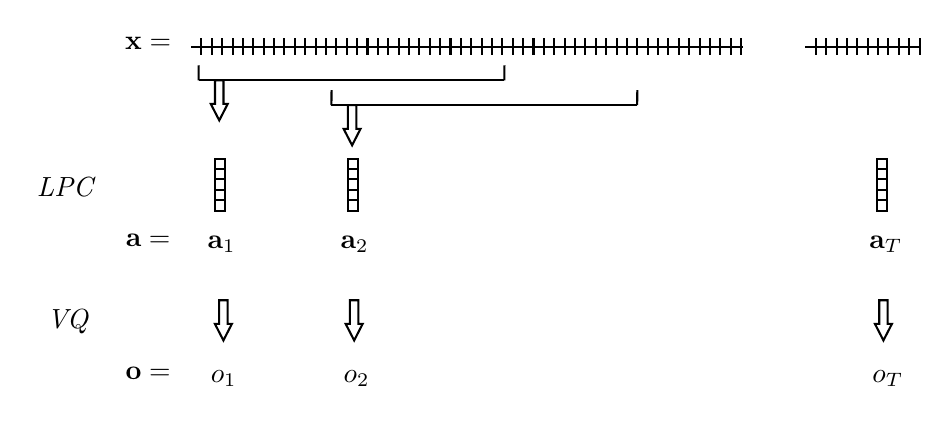
\begin{tikzpicture}[x=0.75pt,y=0.75pt,yscale=-1,xscale=1]
    %uncomment if require: \path (0,450); %set diagram left start at 0, and has height of 450

    %Straight Lines [id:da01594281834627176]
    \draw    (80.33,6.78) -- (346.26,6.78) (85.33,2.78) -- (85.33,10.78)(90.33,2.78) -- (90.33,10.78)(95.33,2.78) -- (95.33,10.78)(100.33,2.78) -- (100.33,10.78)(105.33,2.78) -- (105.33,10.78)(110.33,2.78) -- (110.33,10.78)(115.33,2.78) -- (115.33,10.78)(120.33,2.78) -- (120.33,10.78)(125.33,2.78) -- (125.33,10.78)(130.33,2.78) -- (130.33,10.78)(135.33,2.78) -- (135.33,10.78)(140.33,2.78) -- (140.33,10.78)(145.33,2.78) -- (145.33,10.78)(150.33,2.78) -- (150.33,10.78)(155.33,2.78) -- (155.33,10.78)(160.33,2.78) -- (160.33,10.78)(165.33,2.78) -- (165.33,10.78)(170.33,2.78) -- (170.33,10.78)(175.33,2.78) -- (175.33,10.78)(180.33,2.78) -- (180.33,10.78)(185.33,2.78) -- (185.33,10.78)(190.33,2.78) -- (190.33,10.78)(195.33,2.78) -- (195.33,10.78)(200.33,2.78) -- (200.33,10.78)(205.33,2.78) -- (205.33,10.78)(210.33,2.78) -- (210.33,10.78)(215.33,2.78) -- (215.33,10.78)(220.33,2.78) -- (220.33,10.78)(225.33,2.78) -- (225.33,10.78)(230.33,2.78) -- (230.33,10.78)(235.33,2.78) -- (235.33,10.78)(240.33,2.78) -- (240.33,10.78)(245.33,2.78) -- (245.33,10.78)(250.33,2.78) -- (250.33,10.78)(255.33,2.78) -- (255.33,10.78)(260.33,2.78) -- (260.33,10.78)(265.33,2.78) -- (265.33,10.78)(270.33,2.78) -- (270.33,10.78)(275.33,2.78) -- (275.33,10.78)(280.33,2.78) -- (280.33,10.78)(285.33,2.78) -- (285.33,10.78)(290.33,2.78) -- (290.33,10.78)(295.33,2.78) -- (295.33,10.78)(300.33,2.78) -- (300.33,10.78)(305.33,2.78) -- (305.33,10.78)(310.33,2.78) -- (310.33,10.78)(315.33,2.78) -- (315.33,10.78)(320.33,2.78) -- (320.33,10.78)(325.33,2.78) -- (325.33,10.78)(330.33,2.78) -- (330.33,10.78)(335.33,2.78) -- (335.33,10.78)(340.33,2.78) -- (340.33,10.78)(345.33,2.78) -- (345.33,10.78) ;


    %Shape: Grid [id:dp23348643338301867]
    \draw  [draw opacity=0] (91.83,60.78) -- (96.83,60.78) -- (96.83,85.78) -- (91.83,85.78) -- cycle ; \draw    ; \draw   (91.83,65.78) -- (96.83,65.78)(91.83,70.78) -- (96.83,70.78)(91.83,75.78) -- (96.83,75.78)(91.83,80.78) -- (96.83,80.78) ; \draw   (91.83,60.78) -- (96.83,60.78) -- (96.83,85.78) -- (91.83,85.78) -- cycle ;
    %Straight Lines [id:da18845328084567692]
    \draw    (83.96,23) -- (231.27,23) ;


    %Straight Lines [id:da22066749517532758]
    \draw    (83.96,23) -- (84.02,15.78) ;


    %Straight Lines [id:da17781894400268783]
    \draw    (231.27,23) -- (231.33,15.78) ;



    %Down Arrow [id:dp1641348319045337]
    \draw   (89.83,34.38) -- (91.87,34.38) -- (91.87,23) -- (95.96,23) -- (95.96,34.38) -- (98,34.38) -- (93.92,42.33) -- cycle ;
    %Shape: Grid [id:dp5596357312856071]
    \draw  [draw opacity=0] (155.83,60.78) -- (160.83,60.78) -- (160.83,85.78) -- (155.83,85.78) -- cycle ; \draw    ; \draw   (155.83,65.78) -- (160.83,65.78)(155.83,70.78) -- (160.83,70.78)(155.83,75.78) -- (160.83,75.78)(155.83,80.78) -- (160.83,80.78) ; \draw   (155.83,60.78) -- (160.83,60.78) -- (160.83,85.78) -- (155.83,85.78) -- cycle ;
    %Shape: Grid [id:dp23574651045711348]
    \draw  [draw opacity=0] (410.83,60.78) -- (415.83,60.78) -- (415.83,85.78) -- (410.83,85.78) -- cycle ; \draw    ; \draw   (410.83,65.78) -- (415.83,65.78)(410.83,70.78) -- (415.83,70.78)(410.83,75.78) -- (415.83,75.78)(410.83,80.78) -- (415.83,80.78) ; \draw   (410.83,60.78) -- (415.83,60.78) -- (415.83,85.78) -- (410.83,85.78) -- cycle ;
    %Straight Lines [id:da5803547653809475]
    \draw    (147.96,35) -- (295.27,35) ;


    %Straight Lines [id:da7303303253711202]
    \draw    (147.96,35) -- (148.02,27.78) ;


    %Straight Lines [id:da7587981770652479]
    \draw    (295.27,35) -- (295.33,27.78) ;



    %Down Arrow [id:dp8762704300541813]
    \draw   (153.83,46.38) -- (155.87,46.38) -- (155.87,35) -- (159.96,35) -- (159.96,46.38) -- (162,46.38) -- (157.92,54.33) -- cycle ;
    %Down Arrow [id:dp14503895036340997]
    \draw   (91.83,140.38) -- (93.87,140.38) -- (93.87,129) -- (97.96,129) -- (97.96,140.38) -- (100,140.38) -- (95.92,148.33) -- cycle ;
    %Down Arrow [id:dp3912637147310176]
    \draw   (154.83,140.38) -- (156.87,140.38) -- (156.87,129) -- (160.96,129) -- (160.96,140.38) -- (163,140.38) -- (158.92,148.33) -- cycle ;
    %Down Arrow [id:dp4181538705775292]
    \draw   (409.83,140.38) -- (411.88,140.38) -- (411.88,129) -- (415.96,129) -- (415.96,140.38) -- (418,140.38) -- (413.92,148.33) -- cycle ;
    %Straight Lines [id:da42116590265986353]
    \draw    (376.33,6.78) -- (431.76,6.78) (381.33,2.78) -- (381.33,10.78)(386.33,2.78) -- (386.33,10.78)(391.33,2.78) -- (391.33,10.78)(396.33,2.78) -- (396.33,10.78)(401.33,2.78) -- (401.33,10.78)(406.33,2.78) -- (406.33,10.78)(411.33,2.78) -- (411.33,10.78)(416.33,2.78) -- (416.33,10.78)(421.33,2.78) -- (421.33,10.78)(426.33,2.78) -- (426.33,10.78)(431.33,2.78) -- (431.33,10.78) ;



    % Text Node
    \draw (59.67,5.07) node   {$\mathbf{x} =$};
    % Text Node
    \draw (95.07,101.87) node   {$\mathbf{a}_{1}$};
    % Text Node
    \draw (159.07,101.87) node   {$\mathbf{a}_{2}$};
    % Text Node
    \draw (236.07,161.87) node   {$\dotsc $};
    % Text Node
    \draw (415.07,101.87) node   {$\mathbf{a}_{T}$};
    % Text Node
    \draw (362.73,4.2) node   {$\dotsc $};
    % Text Node
    \draw (20.5,74.5) node  [align=left] {\textit{LPC}};
    % Text Node
    \draw (96.07,166.87) node   {$o_{1}$};
    % Text Node
    \draw (160.07,166.87) node   {$o_{2}$};
    % Text Node
    \draw (416.07,166.87) node   {$o_{T}$};
    % Text Node
    \draw (21.5,139.5) node  [align=left] {\textit{VQ}};
    % Text Node
    \draw (236.07,97.87) node   {$\dotsc $};
    % Text Node
    \draw (59.67,100.07) node   {$\mathbf{a} =$};
    % Text Node
    \draw (59.67,164.07) node   {$\mathbf{o} =$};


\end{tikzpicture}
